\documentclass[italian,10pt,a4paper]{article}
\usepackage[T1]{fontenc}
\usepackage{graphicx}
\usepackage{geometry}
\usepackage{mathtools}
\usepackage{amssymb}
\usepackage{amsthm}
\usepackage{mathtools}
\usepackage{xcolor}
\usepackage{babel}
\usepackage{listings}
\usepackage{hyperref}
\usepackage{cleveref}
\usepackage{soul}
\usepackage{semantic}
%\lstset{
%	basicstyle=\footnotesize\ttfamily,
%	mathescape, 
%	tabsize=4,
%	breakatwhitespace,
%	breaklines,
%	breakautoindent,
%	escapeinside={§}{§},
%	numbers=left,
%	numberstyle=\tiny
%}
\lstset{
language=C++,
basicstyle=\footnotesize\ttfamily,
keywordstyle=\color{blue},
commentstyle=\color{green},
stringstyle=\color{red},
numbers=left,
numberstyle=\tiny,
frame=none,
backgroundcolor=\color{gray!5},
breaklines=true,
tabsize=2
}
\author{Riccardo Torre}
\title{Algoritmi}
\begin{document}
	\maketitle
	\tableofcontents
	\section{Strutture dati}
	\subsection{Stack minimo/coda minima}
	\subsubsection{Modifica dello stack}
	Per trovare l'elemento più piccolo in uno stack in $O(1)$ mantenendo il comportamento asintotico per aggiunta e rimozione di elementi, si memorizzano delle coppie. 
	\begin{figure}[tbph]
		\centering
		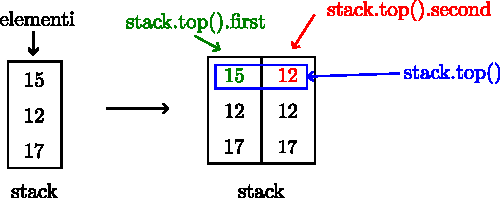
\includegraphics[width=0.7\linewidth]{stack-min-el}
		\caption{l'elemento minimo viene calcolato ad ogni inserimento e salvato sulla seconda colonna dell'elemento in cima allo stack (in rosso).}
		\label{fig:stack-min-el}
	\end{figure}
	\paragraph{Aggiungere un elemento}
	\begin{lstlisting}[caption={aggiungere un elemento.}]
		int new_min = st.empty() ? new_elem : min(new_elem, st.top().second);
		st.push({new_elem, new_min});
	\end{lstlisting}
	\begin{lstlisting}[caption={rimuovere un elemento.}]
		int removed_element = st.top().first;
		st.pop();
	\end{lstlisting}
	\begin{lstlisting}[caption={trovare il minimo.}]
		int minimum = st.top().second;
	\end{lstlisting}Lo stack ha un comportamento LIFO.
	\subsubsection{Modifica della coda -- metodo 1}La coda ha un comportamento FIFO. Non memorizza tutti gli elementi: vengono memorizzati solo quelli necessari per determinare il minimo. La coda viene mantenuta in \textit{ordine non decrescente}\footnote{cioè $\forall i \in [0,\texttt{coda.length}()-1]\colon \texttt{coda[i]} \le \texttt{coda[i+1]}$} (il valore più piccolo sarà memorizzato nella testa). Il minimo effettivo deve sempre essere mantenuto nella coda. 
	
	Prima di aggiungere un nuovo elemento nella coda è sufficiente effettuare un ``taglio'': vengono rimossi tutti gli elementi finali della coda che sono più grandi del nuovo elemento e successivamente si aggiunge il nuovo elemento alla coda. In questo modo viene mantenuto l'ordine non decrescente e non viene perso l'elemento corrente se in qualsiasi passaggio successivo è l'elemento minimo. Tutti gli elementi che vengono rimossi non potranno mai essere primi. 
	
	Quando si vuole estrarre un elemento dalla testa, potrebbe non essere presente se è stato rimosso in precedenza con un elemento più piccolo. Pertanto quando si elimina un elemento da una coda bisogna conoscerne il valore. Se la testa della coda ha lo stesso valore, può essere rimossa in sicurezza, altrimenti non viene apportata nessuna modifica.
	\begin{lstlisting}[caption={implementazione della coda.}]
		deque<int> 1;
	\end{lstlisting}

\begin{lstlisting}[caption={trovare il minimo.}]
	int minimum = q.front();
\end{lstlisting}
\begin{lstlisting}[caption={aggiungere un elemento.}]
	while (!q.empty() && q.back() > new_element)
	q.pop_back();
	q.push_back(new_element);
\end{lstlisting}
\begin{lstlisting}[caption={rimuovere un elemento.}]
	if (!q.empty() && q.front() == remove_element)
	q.pop_front();
\end{lstlisting}
\end{document}